\question \textbf{Bitvectors}
Proof the statement on slide 2059 is true:
\begin{equation}
\begin{pmatrix}
b\\c
\end{pmatrix}
\cdot
\begin{pmatrix}
b\\c'
\end{pmatrix}
\leq
\begin{pmatrix}
2\cdot b\\c + c'
\end{pmatrix}
\end{equation}



\begin{solution}

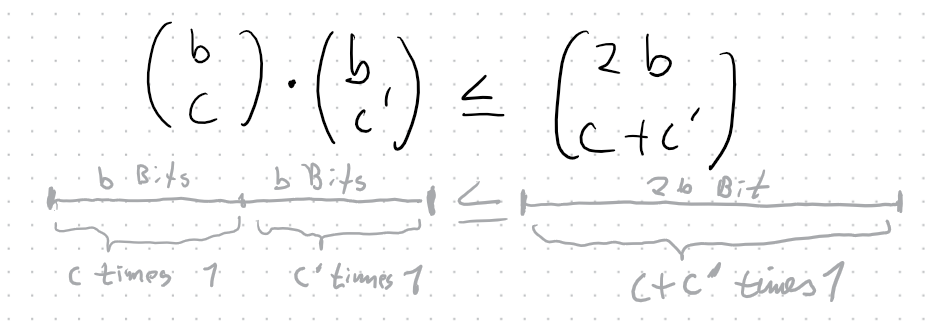
\includegraphics[width=0.5\linewidth]{task_3/a3.png}

The left side of the inequality is the number of possible $2b$ long bitvectors with $c$ 1s in the left half and $c'$ 1s in the right half. The right side of the inequality is the number of possible $2b$ long bitvectors in with $c+c'$ 1s in total. So the inequality is obviously true, because the bitvectors with $c$ 1s in the left and $c'$ 1s in the right half are a subset of the bitvectors with $c+c'$ 1s in total.
\end{solution}